% the following command is only required if the thesis is written in german
\RequirePackage[ngerman=ngerman-x-latest]{hyphsubst}

\documentclass[
  ngerman, % change to ngerman for german theses
  symmetric, % use two-side for booklike layouts
  cdfont=off, % modify this to use the TUD font (Open Sans)
  numbers=noenddot % remove trailing dots in chapter/section/... enumeration
]{tudscrreprt}
% use a custom serif font
\usepackage[bitstream-charter]{mathdesign}
% make chapter, section, ... use serif font
\addtokomafont{disposition}{\rmfamily}

\usepackage[T1]{fontenc}
\usepackage[utf8]{inputenc}
\usepackage[
  ngerman % change to ngerman for german theses
]{babel}
\usepackage{isodate}
\usepackage{pdfpages}
\usepackage{listings}
\usepackage[toc, page]{appendix}
\usepackage{hyphenat}

\usepackage[
  style=alphabetic,
  backend=biber,
  url=false,
  doi=false,
  isbn=false,
  hyperref,
]{biblatex}
% configure the location of the biblatex file
\addbibresource{bibliography.bib}
\AtEveryBibitem{%
  \clearfield{note}%
}

% make all links clickable but hide ugly boxes
\usepackage[hidelinks]{hyperref}
% automatically insert Fig. X in the text with \cref{..}
\usepackage[capitalise,nameinlink,noabbrev]{cleveref}

\usepackage[colorinlistoftodos,prependcaption,textsize=tiny]{todonotes}

\usepackage{graphicx}
\graphicspath{ {./images/} }

\usepackage{svg}

% if you need mathy stuff
\newtheorem{lem}{Lemma}
\crefname{lem}{Lemma}{Lemmas}
\newtheorem{thm}{Theorem}
\crefname{thm}{Theorem}{Theorems}
\newtheorem{defs}{Definition}
\crefname{defs}{Def.}{Defs.}

\usepackage{blindtext}

%\usepackage{tudscrsupervisor} % if you want to copy the sources of the task description into the thesis

\usepackage{csquotes}

\usepackage{caption}
\captionsetup{font=normalfont,labelfont=normalfont,labelsep=space}
\usepackage{floatrow}
\floatsetup{font=normalfont}
\floatsetup[table]{style=plaintop}
\captionsetup{singlelinecheck=off,format=hang,justification=raggedright}
\DeclareCaptionSubType[alph]{figure}
\DeclareCaptionSubType[alph]{table}
\captionsetup[subfloat]{labelformat=brace,list=off}

\usepackage{booktabs}
\usepackage{array}
\usepackage{tabularx}
\usepackage{tabulary}
\usepackage{tabu}
\usepackage{longtable}
\usepackage{multirow}

\usepackage{quoting}

\usepackage[babel]{microtype}

\usepackage{xfrac}

\usepackage{enumitem}
\setlist[itemize]{noitemsep}

\usepackage{ellipsis}
\let\ellipsispunctuation\relax

\usepackage{listings}
\usepackage{xcolor}

\definecolor{commentsColor}{rgb}{0.497495, 0.497587, 0.497464}
\definecolor{keywordsColor}{rgb}{0.000000, 0.000000, 0.635294}
\definecolor{stringColor}{rgb}{0.558215, 0.000000, 0.135316}

\lstset{ %
  backgroundcolor=\color{white},   % choose the background color; you must add \usepackage{color} or \usepackage{xcolor}
  basicstyle=\footnotesize,        % the size of the fonts that are used for the code
  breakatwhitespace=false,         % sets if automatic breaks should only happen at whitespace
  breaklines=true,                 % sets automatic line breaking
  captionpos=b,                    % sets the caption-position to bottom
  commentstyle=\color{commentsColor}\textit,    % comment style
  deletekeywords={...},            % if you want to delete keywords from the given language
  escapeinside={\%*}{*)},          % if you want to add LaTeX within your code
  extendedchars=true,              % lets you use non-ASCII characters; for 8-bits encodings only, does not work with UTF-8
  frame=tb,	                   	   % adds a frame around the code
  keepspaces=true,                 % keeps spaces in text, useful for keeping indentation of code (possibly needs columns=flexible)
  keywordstyle=\color{keywordsColor}\bfseries,       % keyword style
  language=Python,                 % the language of the code (can be overrided per snippet)
  otherkeywords={*,...},           % if you want to add more keywords to the set
  numbers=left,                    % where to put the line-numbers; possible values are (none, left, right)
  numbersep=5pt,                   % how far the line-numbers are from the code
  numberstyle=\tiny\color{commentsColor}, % the style that is used for the line-numbers
  rulecolor=\color{black},         % if not set, the frame-color may be changed on line-breaks within not-black text (e.g. comments (green here))
  showspaces=false,                % show spaces everywhere adding particular underscores; it overrides 'showstringspaces'
  showstringspaces=false,          % underline spaces within strings only
  showtabs=false,                  % show tabs within strings adding particular underscores
  stepnumber=1,                    % the step between two line-numbers. If it's 1, each line will be numbered
  stringstyle=\color{stringColor}, % string literal style
  tabsize=2,	                   % sets default tabsize to 2 spaces
  title=\lstname,                  % show the filename of files included with \lstinputlisting; also try caption instead of title
  columns=fixed                    % Using fixed column width (for e.g. nice alignment)
}

\lstdefinelanguage{XML} % use with language = XML
{
  morestring=[b]",
  morestring=[s]{>}{<},
  morecomment=[s]{<?}{?>},
  morekeywords={xmlns,version,type}
}


 % code styles (listings)

% use this custom theorem for research questions
\newtheorem{researchquestion}{Research Question}
\crefname{researchquestion}{Research Question}{Research Questions}

% use this custom environment for equations
\newenvironment{conditions}
  {\par\vspace{\abovedisplayskip}\noindent\begin{tabular}{>{$}l<{$} @{${}={}$} l}}
  {\end{tabular}\par\vspace{\belowdisplayskip}}

\usepackage{float}

% configure the name of your appendix
\renewcommand\appendixtocname{Appendix}
\renewcommand\appendixpagename{Appendix}

% use \tocless before a chapter/section/... in the
% appendix to hide it from the toc
\newcommand{\nocontentsline}[3]{}
\newcommand{\tocless}[2]{
  \bgroup\let\addcontentsline=\nocontentsline#1{#2}\egroup
}

\begin{document}

  % use uppercase roman letters for all pages until the introduction
  % this way, it is easier to identify how many pages the thesis has
  \pagenumbering{Roman}

  \faculty{Fakultät Informatik}
  \department{}
  \institute{TODO Institut für Software- und Multimediatechnik}
  \chair{TODO Lehrstuhl für Softwaretechnologie}
  \title{%
  TODO Title of your Thesis.
  }

  \thesis{TODO Diplom} % the type of thesis you want to write

  \author{Markus Wieland}
  \matriculationnumber{4791192}
  \matriculationyear{2018}
  \dateofbirth{9.5.2000}
  \placeofbirth{Chemnitz}

  \course{Diplom Informatik (PO 2010)}

  \supervisor{%
    TODO Dipl. Inf. Max Mustermann
  }
  \professor{ TODOProf. Dr. rer. nat. habil. Max Mustermann}
  \date{1.1.1970} % the date of submission
  \maketitle

  \newpage

  % include the task definition if you want
  % \includepdf[pages=-]{task/task.pdf}
  % \newpage

  % for the order of the following sections please refer to
  % the recommendations for thesis structuring
  \confirmation

  \tableofcontents

  \listoffigures
  \addcontentsline{toc}{chapter}{\listfigurename}

  \listoftables
  \addcontentsline{toc}{chapter}{\listtablename}

  % this is where your thesis lives

  \chapter{Examples}\label{ch:examples}\pagenumbering{arabic}

\todo{Remove this example todo.}

\section{Inline Code, Footnotes and URLs}

This an example text, which shows you, how to use the \texttt{tudscr}\footnote{TUD-Script. \url{https://github.com/tud-cd/tudscr} (Visited on Sept. 15 2020)} template and its components. Feel free to remove this example text or use the provided segments for your thesis.

\section{Research Questions, Inline TODOs, Citations and Referencing}


We'd like to answer the following research goals.\todo[inline]{You may of course write some more text than given in this example.}

\begin{researchquestion}\label{rq:matrix}
Do we live in the Matrix?
\end{researchquestion}

\noindent Feel free to explain the motivation behind your research questions.

\begin{researchquestion}\label{rq:possible}
Based on \cite{gos_2020}, is it actually possible to answer \Cref{rq:matrix} in the first place?
\end{researchquestion}

\noindent This research question is relevant, because it just came to my mind. Pull Request if you have a better example, thanks.

\section{Including Graphics and Paragraphs}

Although this has really nothing to do with the previous sections, take the following as an example of how to include graphics.

\begin{figure}[H]
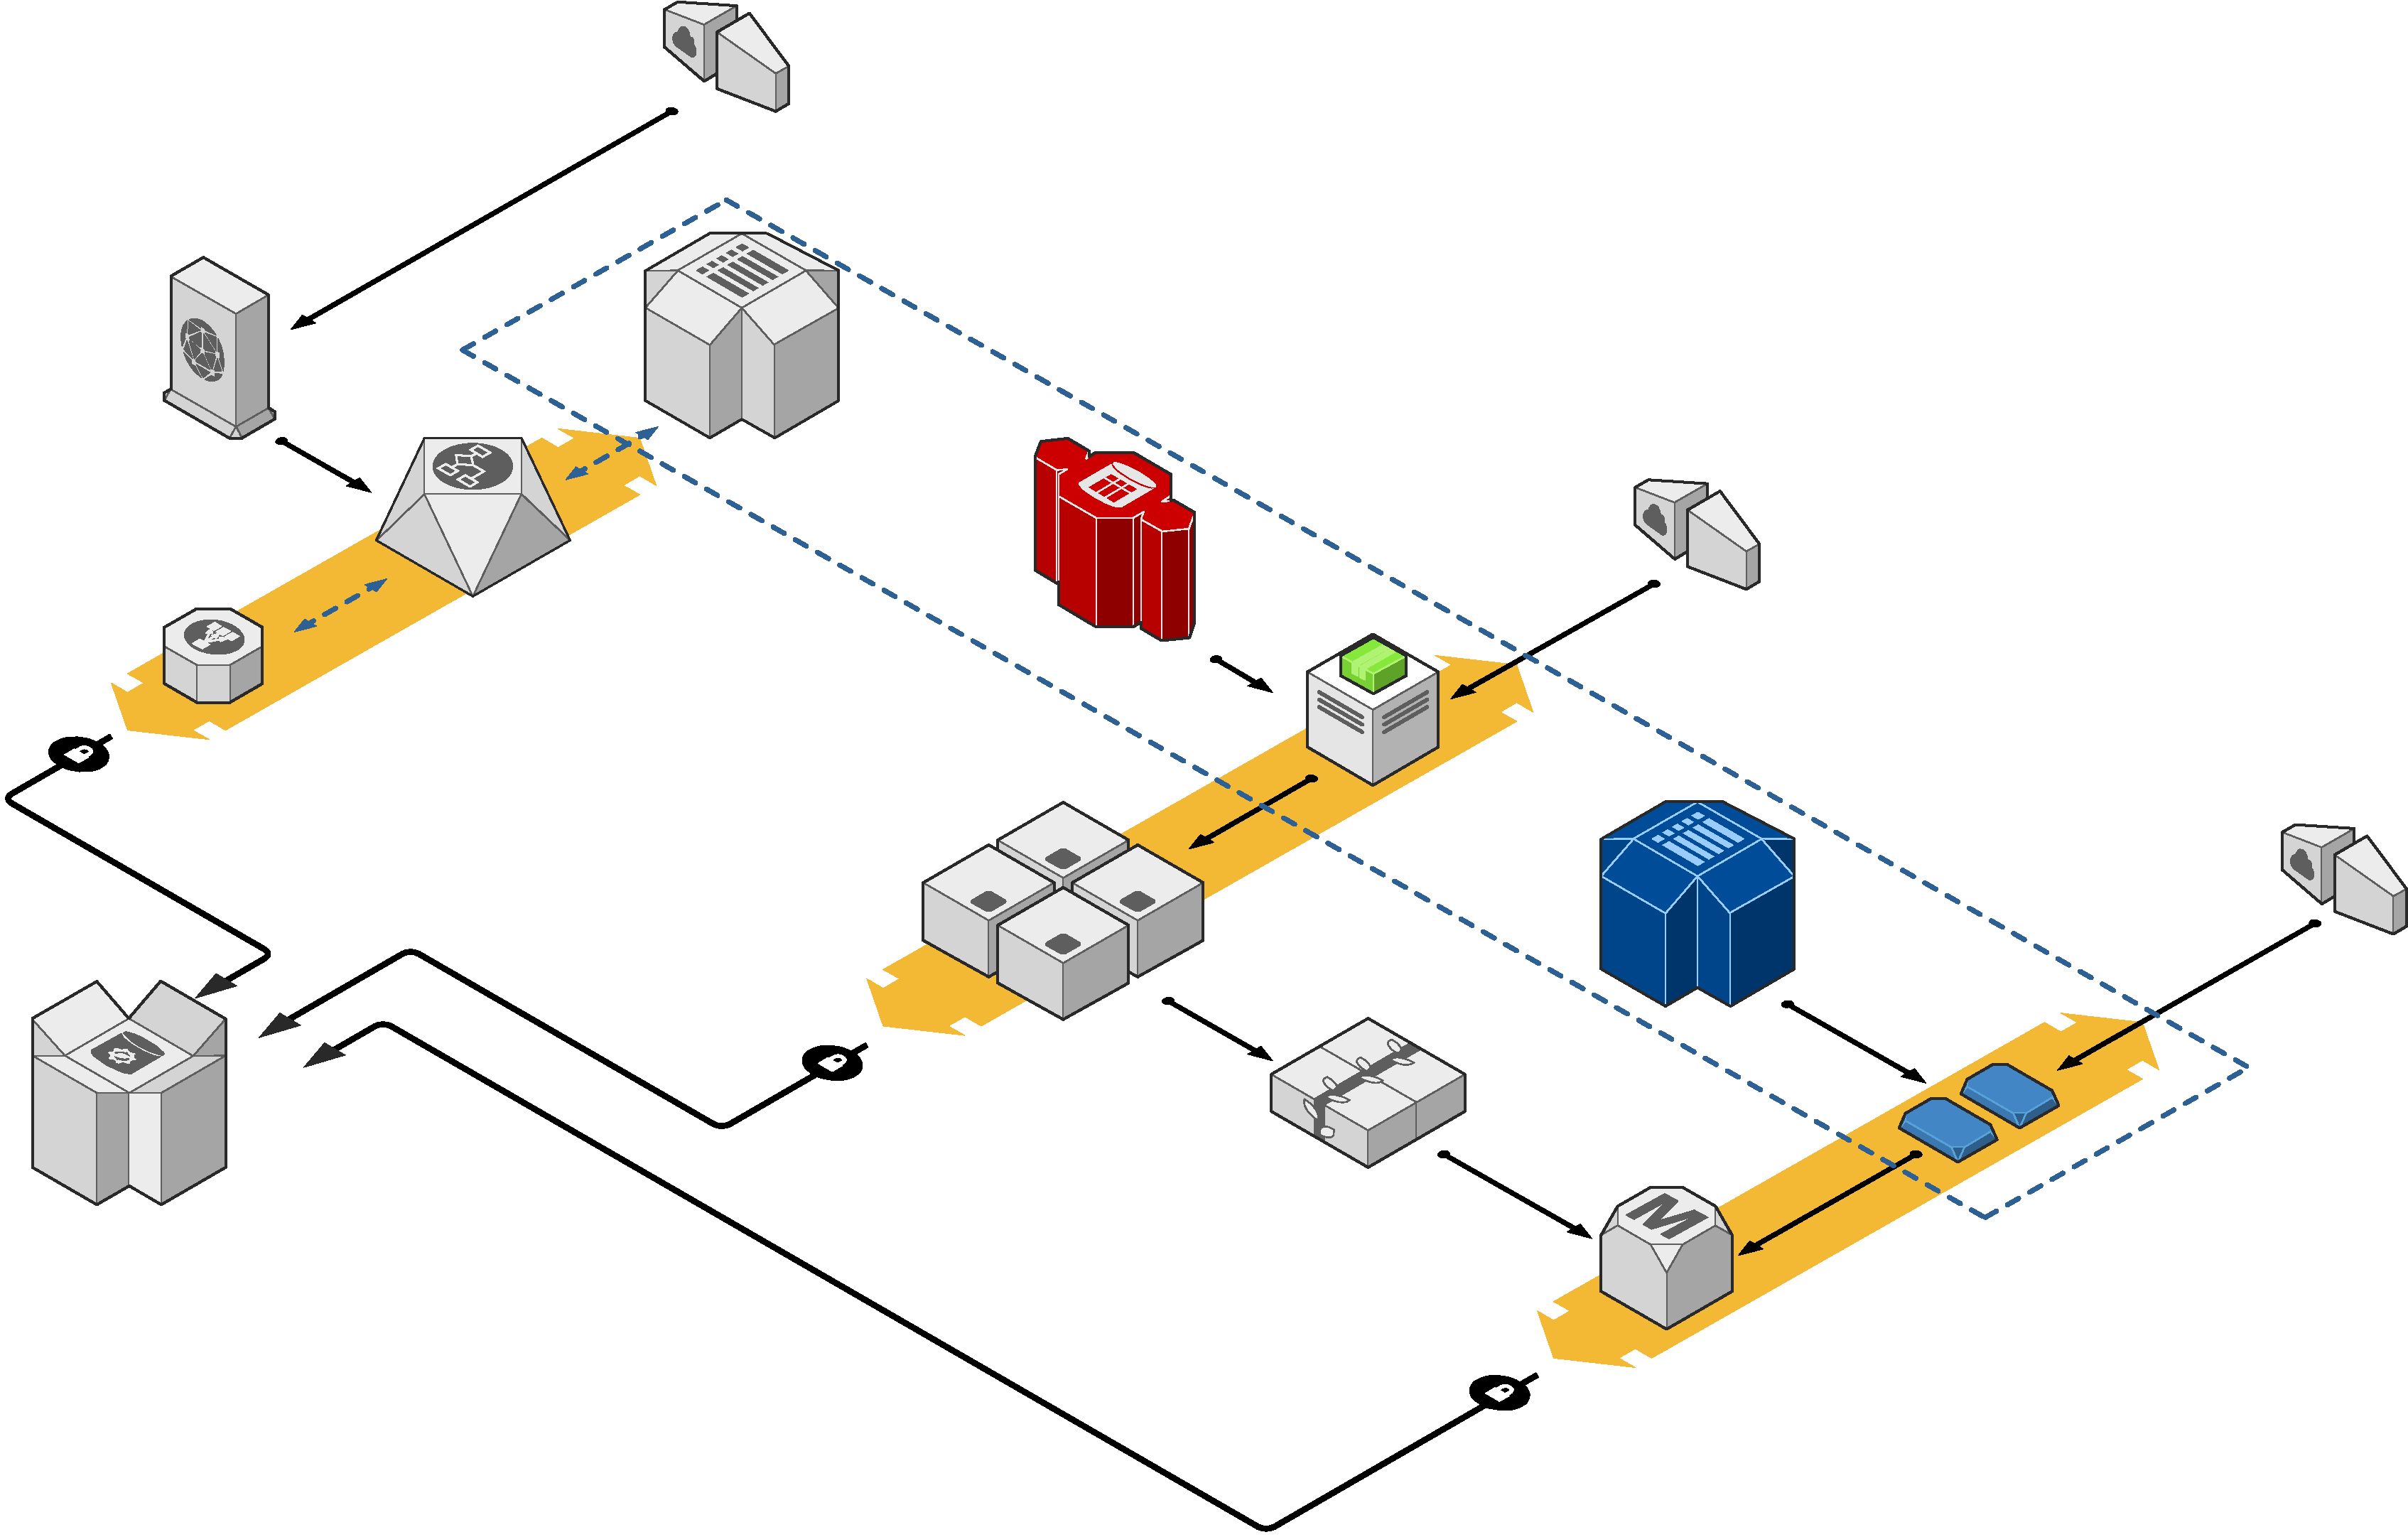
\includegraphics[width=\linewidth, bb=0 0 1626 1038]{example.pdf}
\caption{A really informative diagram following the magical-number-7-principle of Miller \cite{magical_2020}.}\label{fig:example-single}
\end{figure}

\noindent As shown in \Cref{fig:example-single}, including graphics is really easy with PDF files, but you need to give it a \textit{bounding box}, which is simply \texttt{0 0 <width> <height>}. Here is how to include PNG files.

\begin{figure}[H]
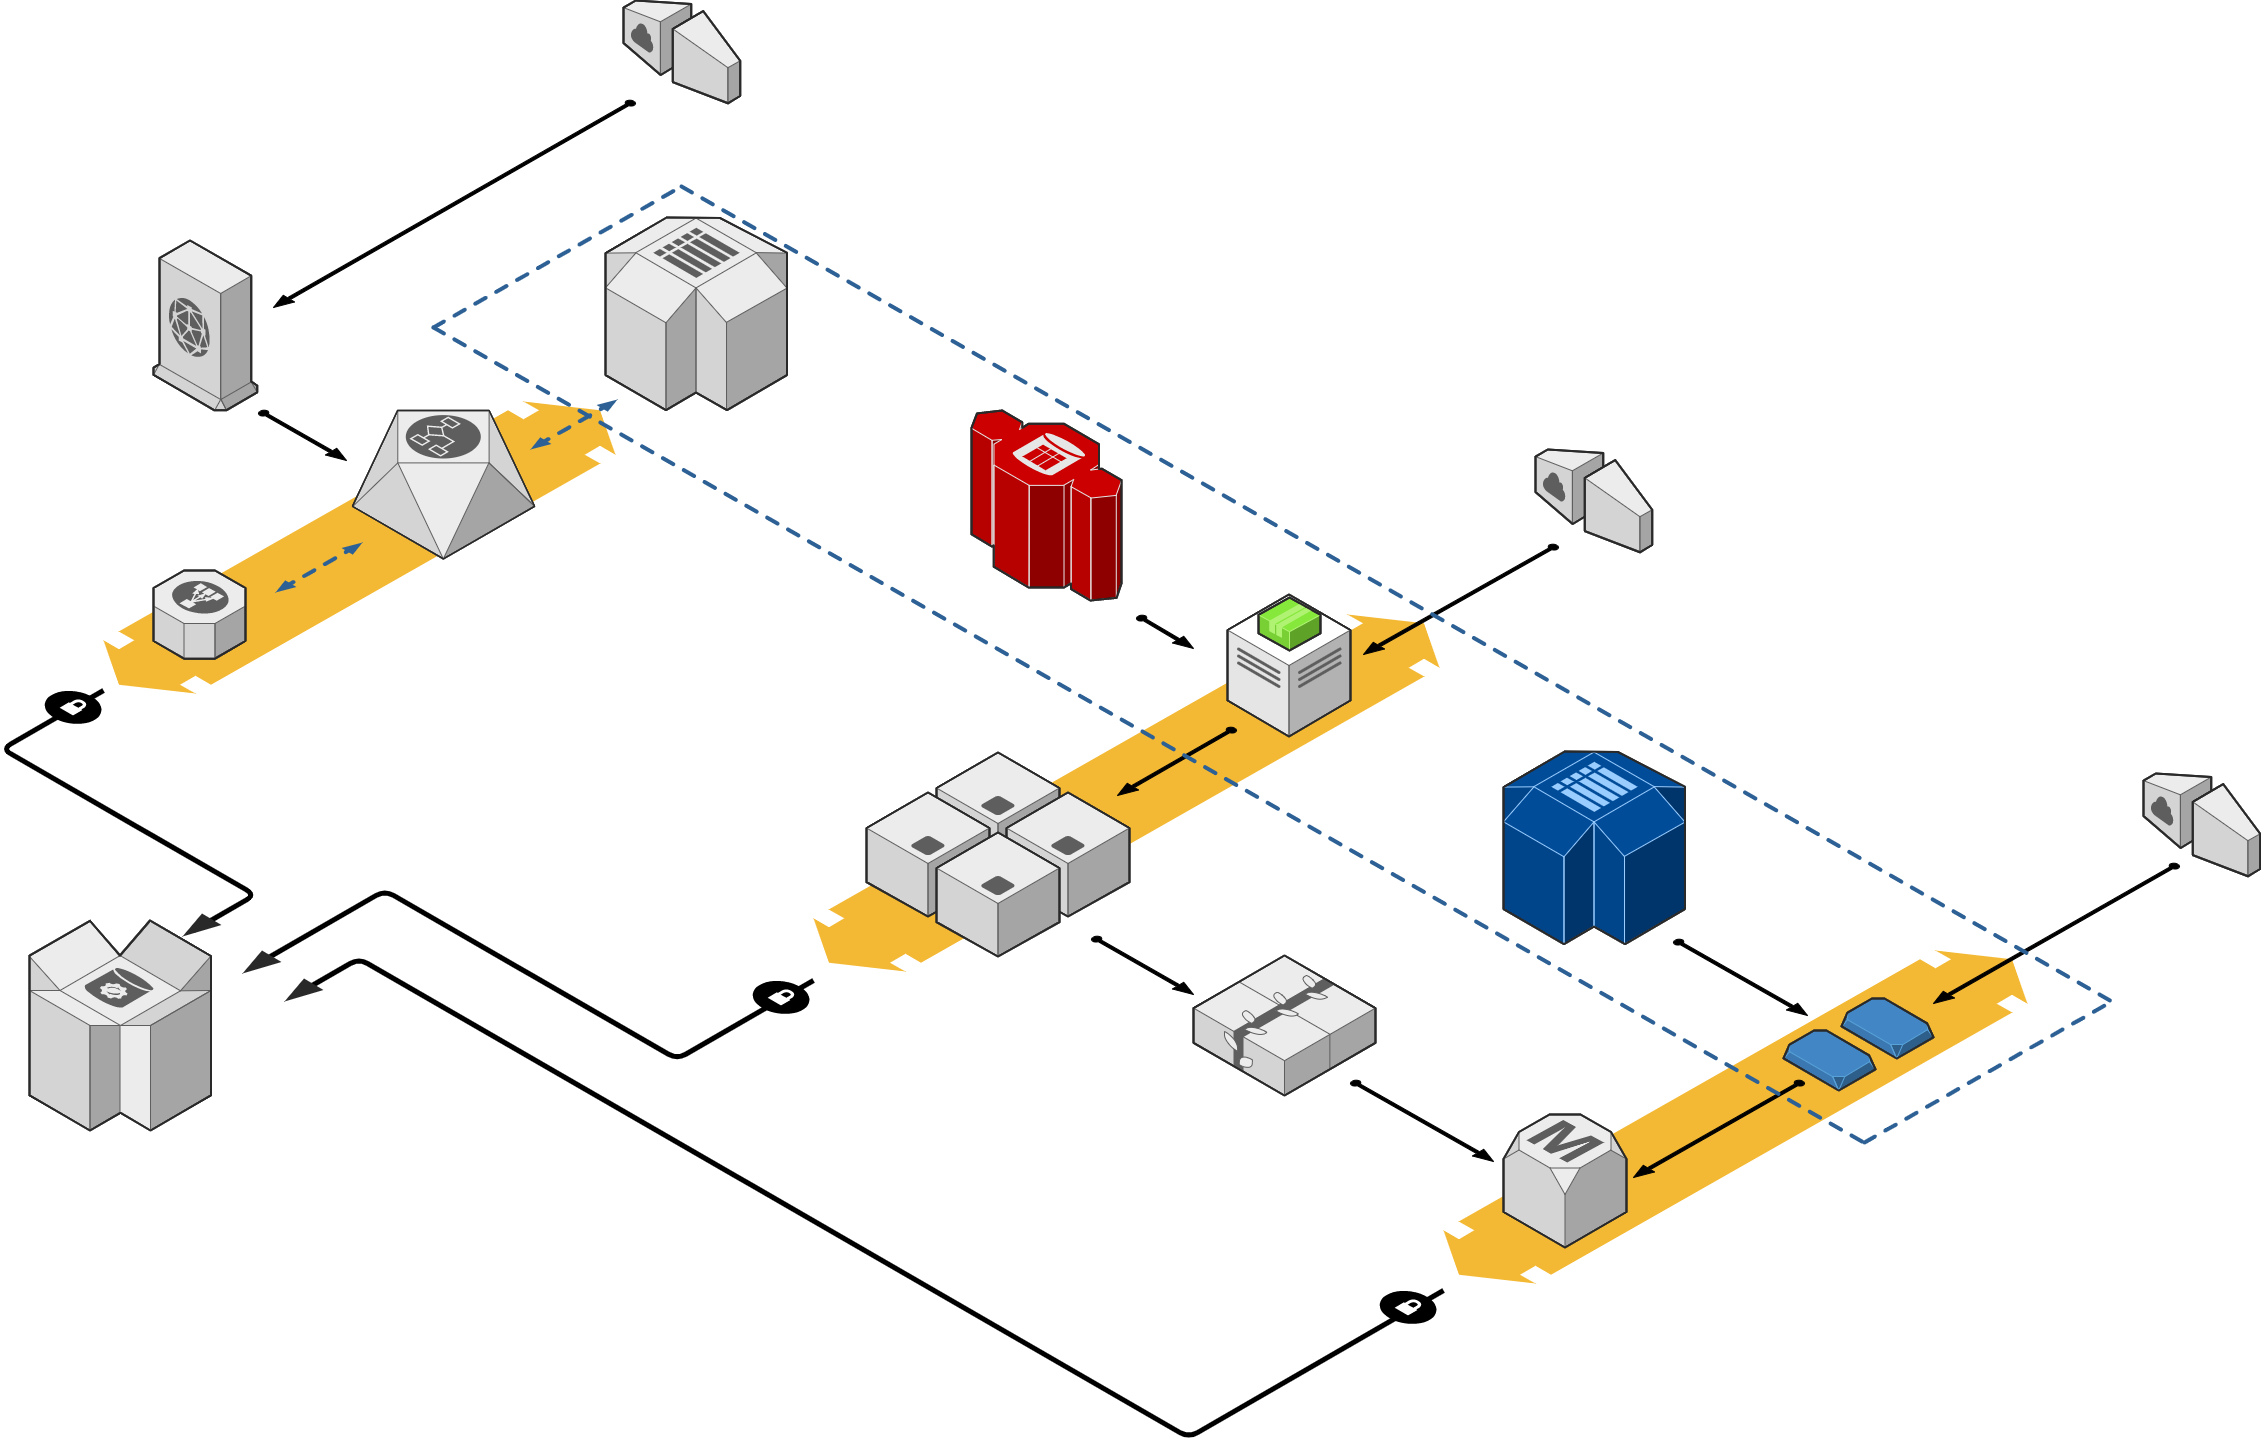
\includegraphics[width=0.75\linewidth]{example.png}
\caption{The same diagram but in PNG and smaller.}\label{fig:example-small}
\end{figure}

\noindent With PNG, no bounding box must be given, but the size of your thesis PDF will probably increase by some order of magnitudes. So try to use PDF whenever possible. Also, avoid JPEG because of the lossy compression. We want our thesis to look nice, or wont we? Try to fiddle around with the option \texttt{H} after the figure, if it doesn't fit the page. This will not be explained here, read the documentation.

\paragraph{One last example:} use the following snippet to include multiple graphics in a table-like structure.

\begin{figure}[H]
\begin{tabular}{ll}
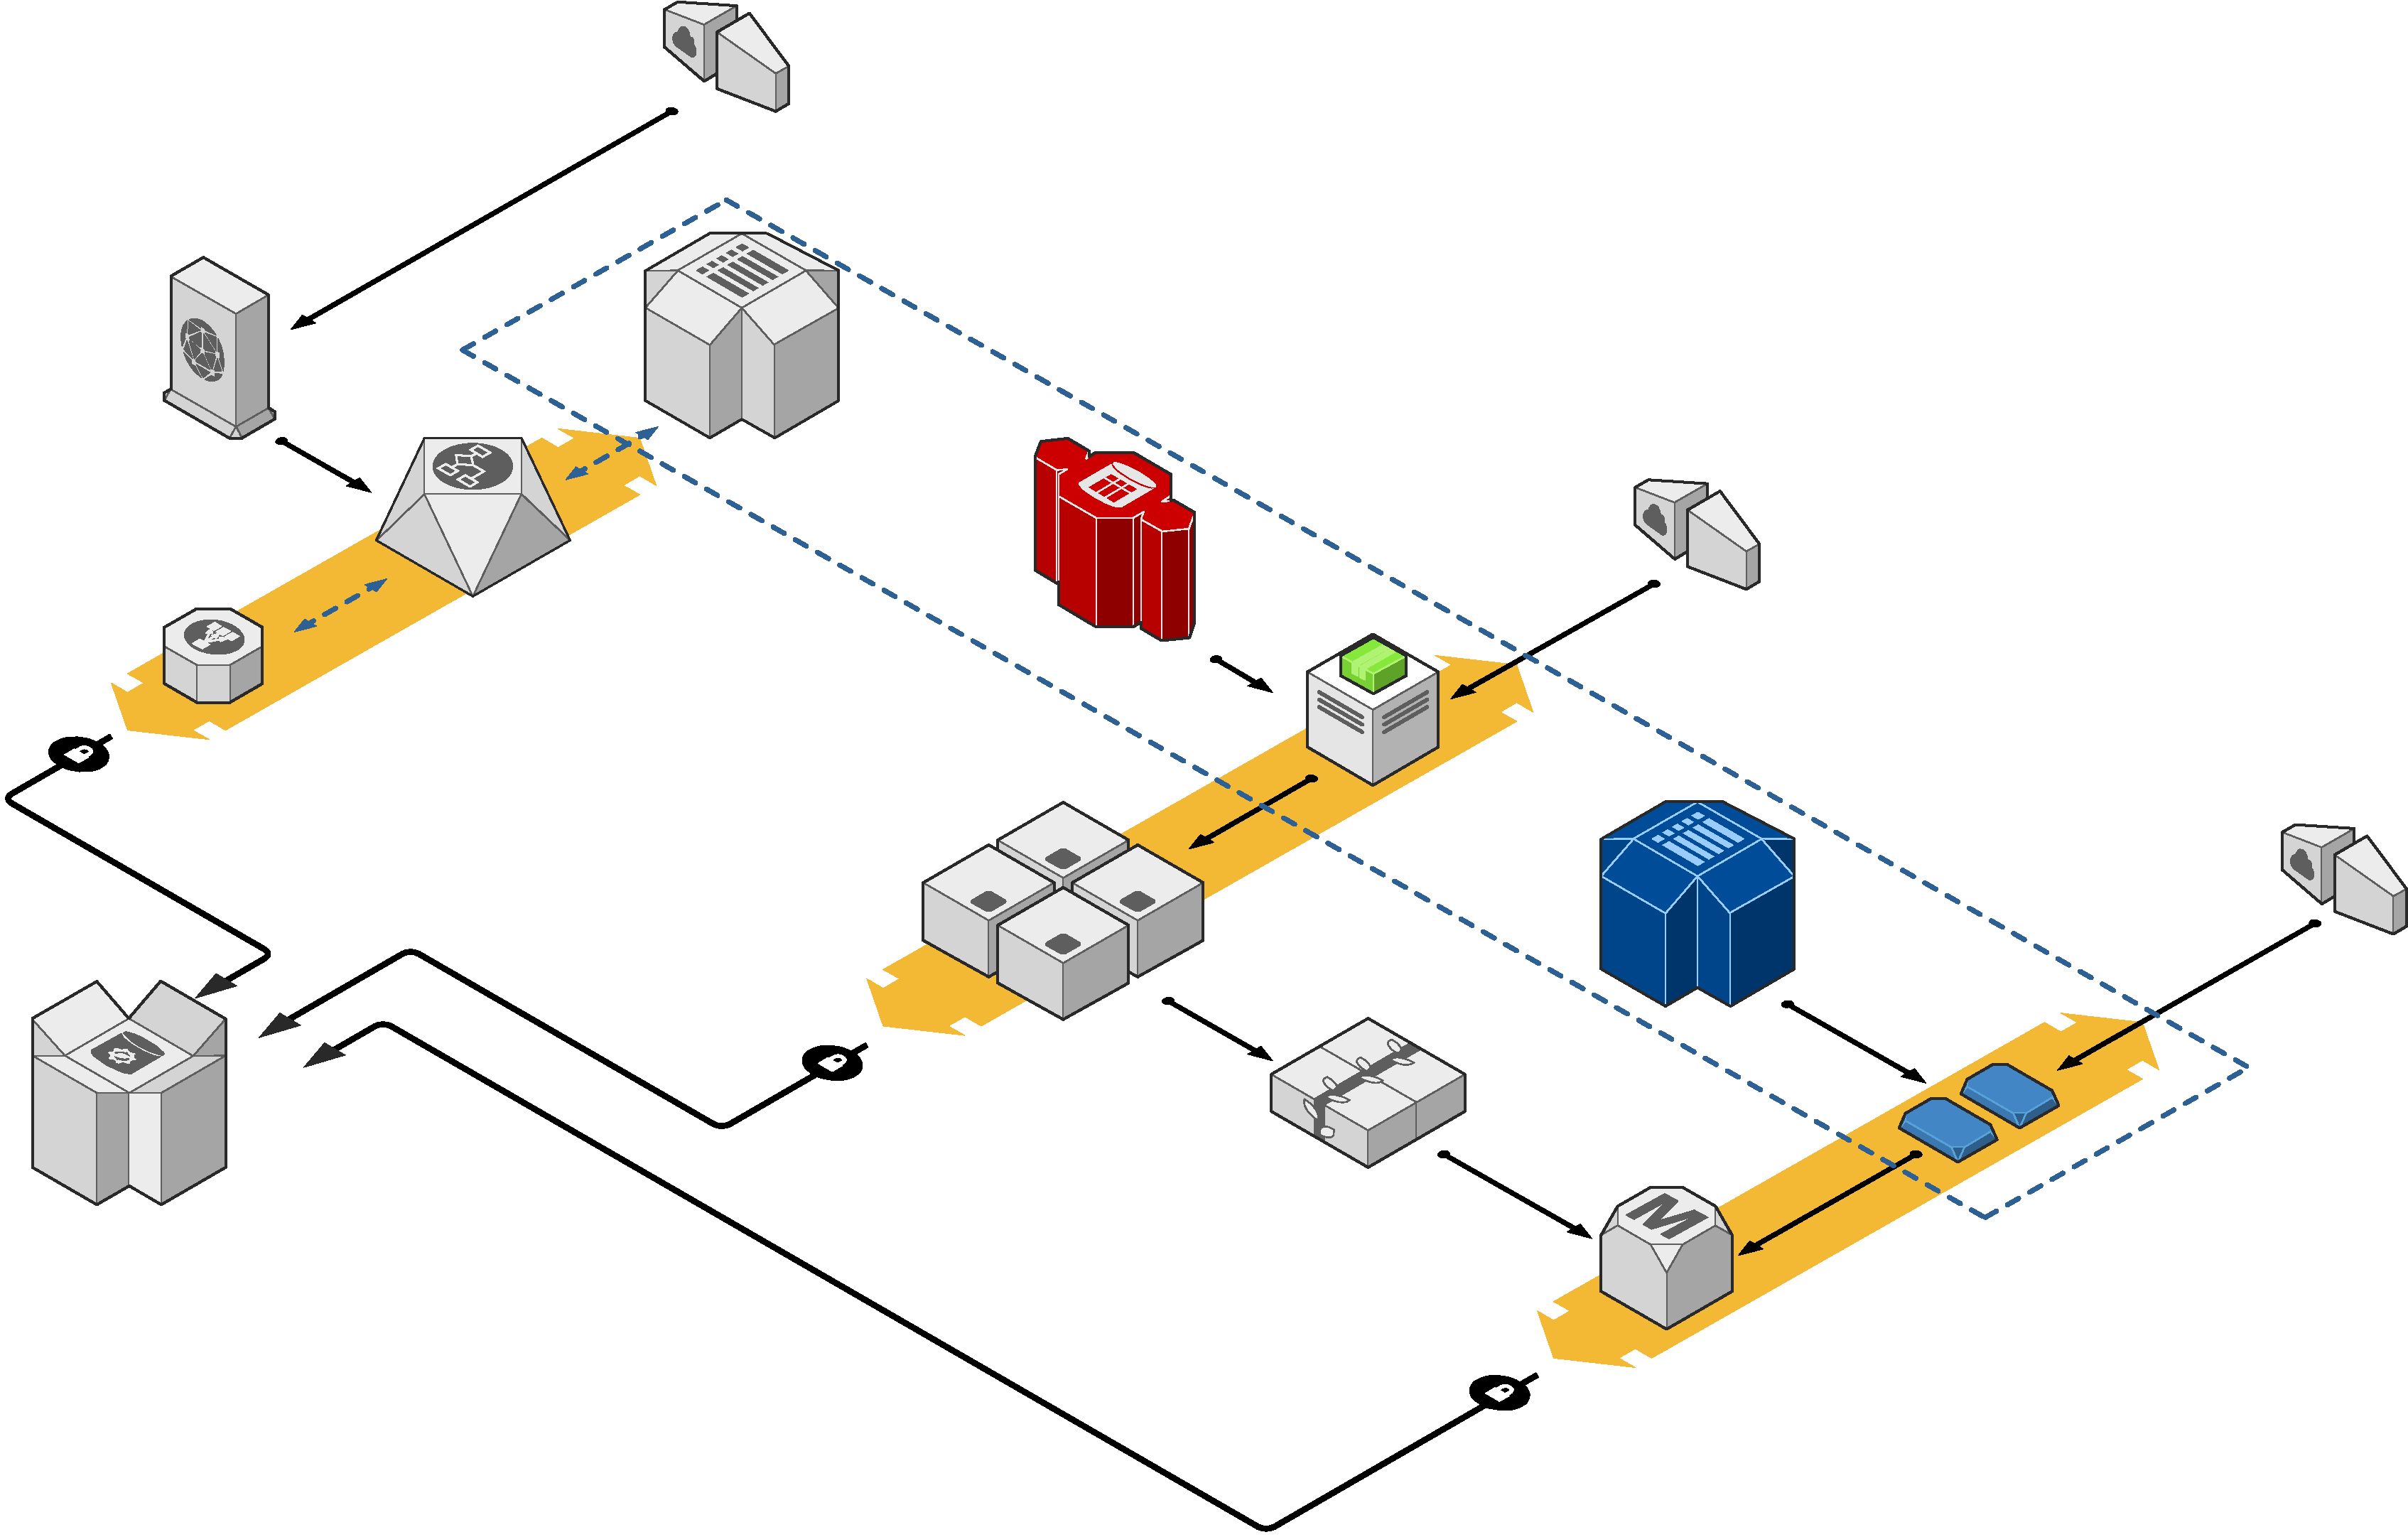
\includegraphics[width=0.4\linewidth, bb=0 0 1626 1038]{example.pdf}
&
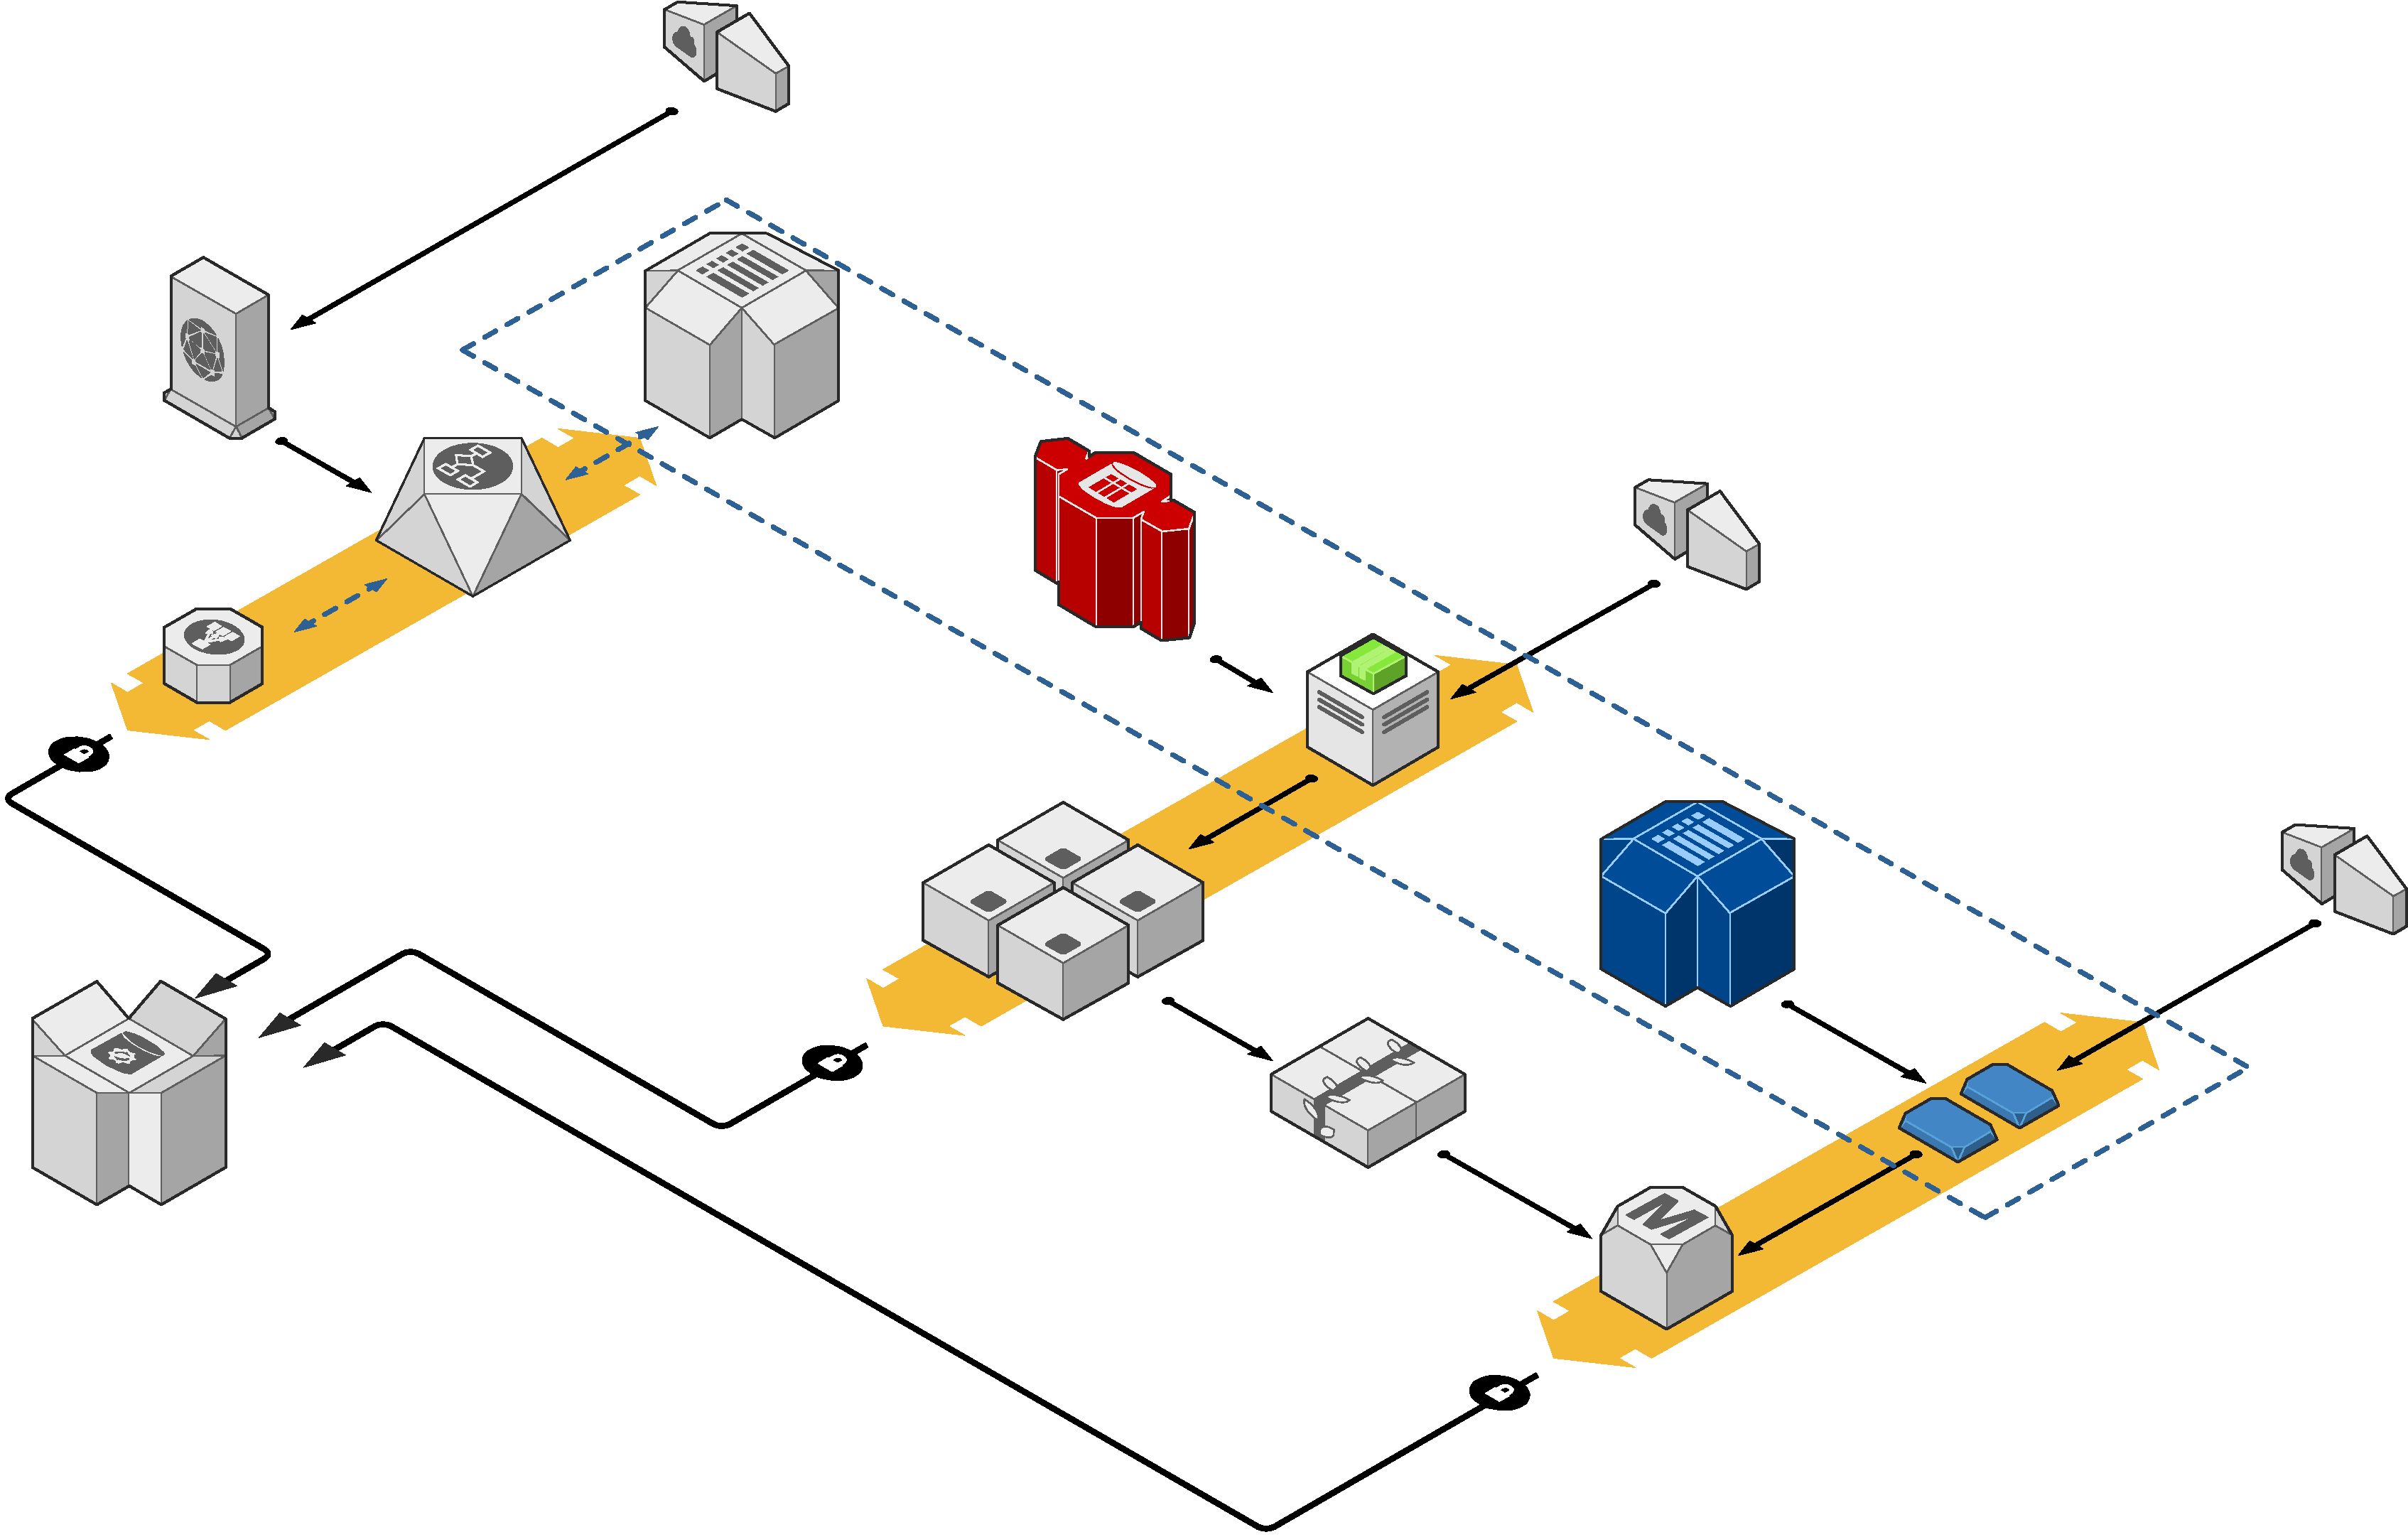
\includegraphics[width=0.4\linewidth, bb=0 0 1626 1038]{example.pdf}
\\
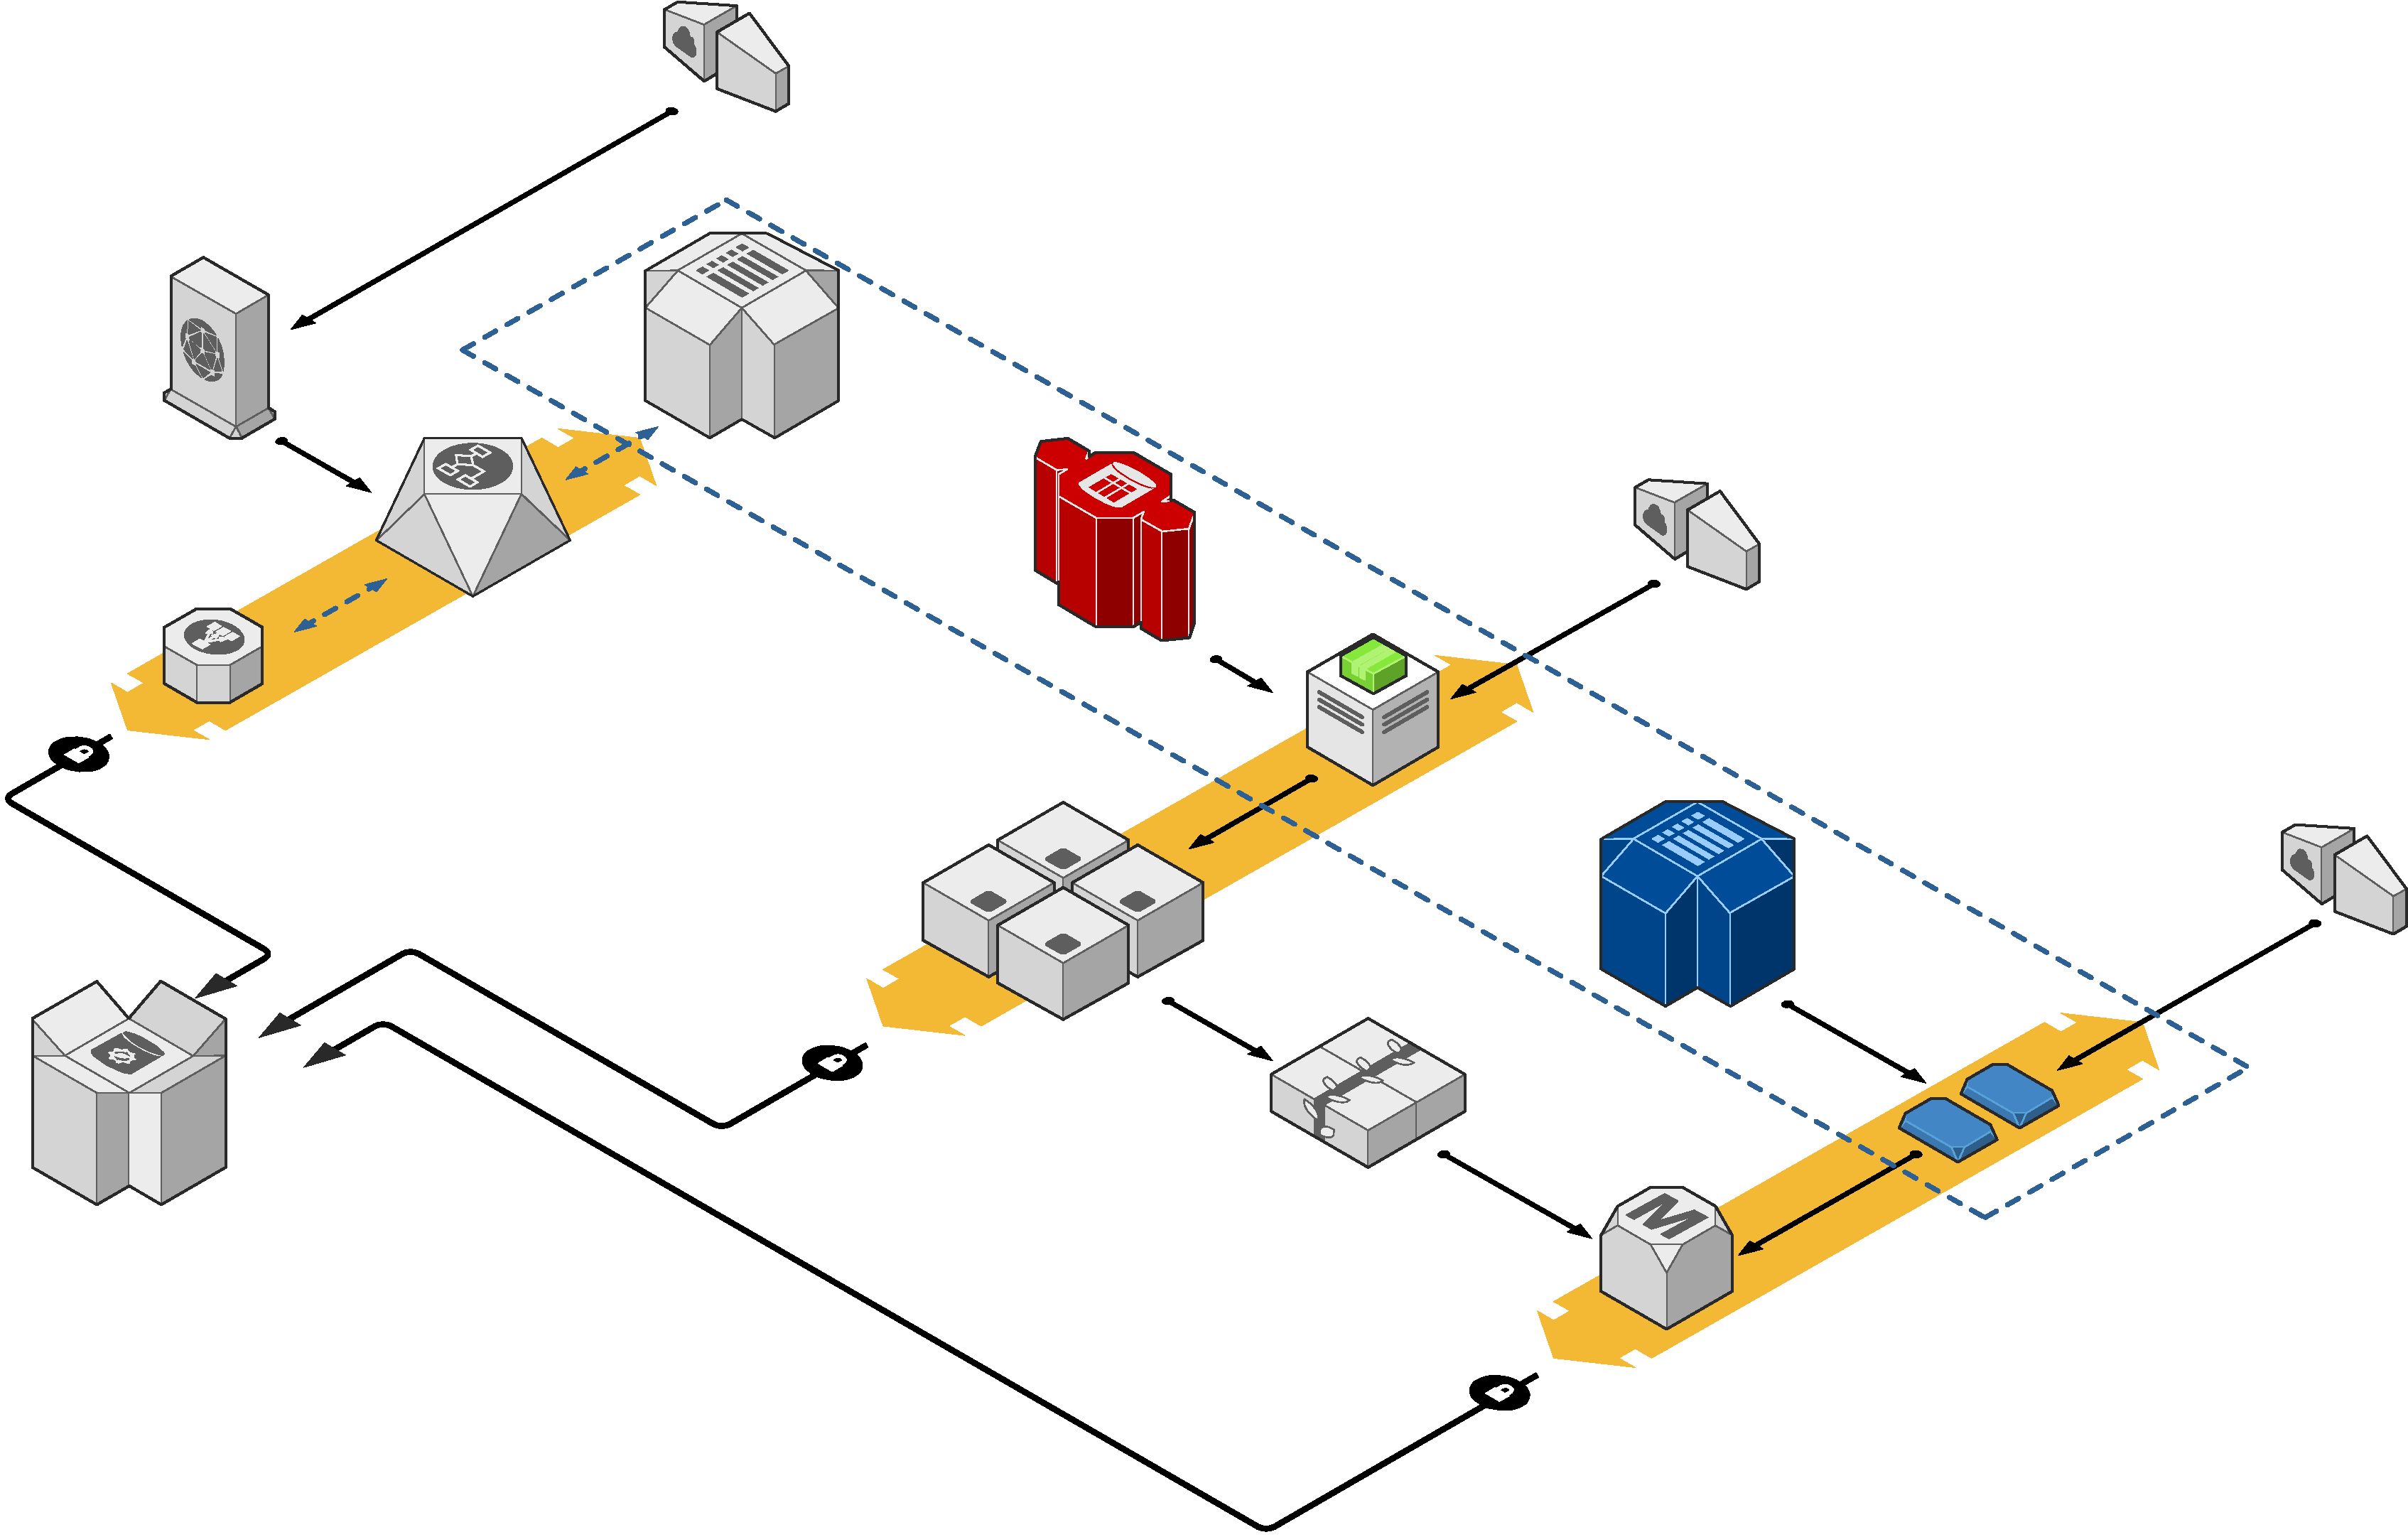
\includegraphics[width=0.4\linewidth, bb=0 0 1626 1038]{example.pdf}
&
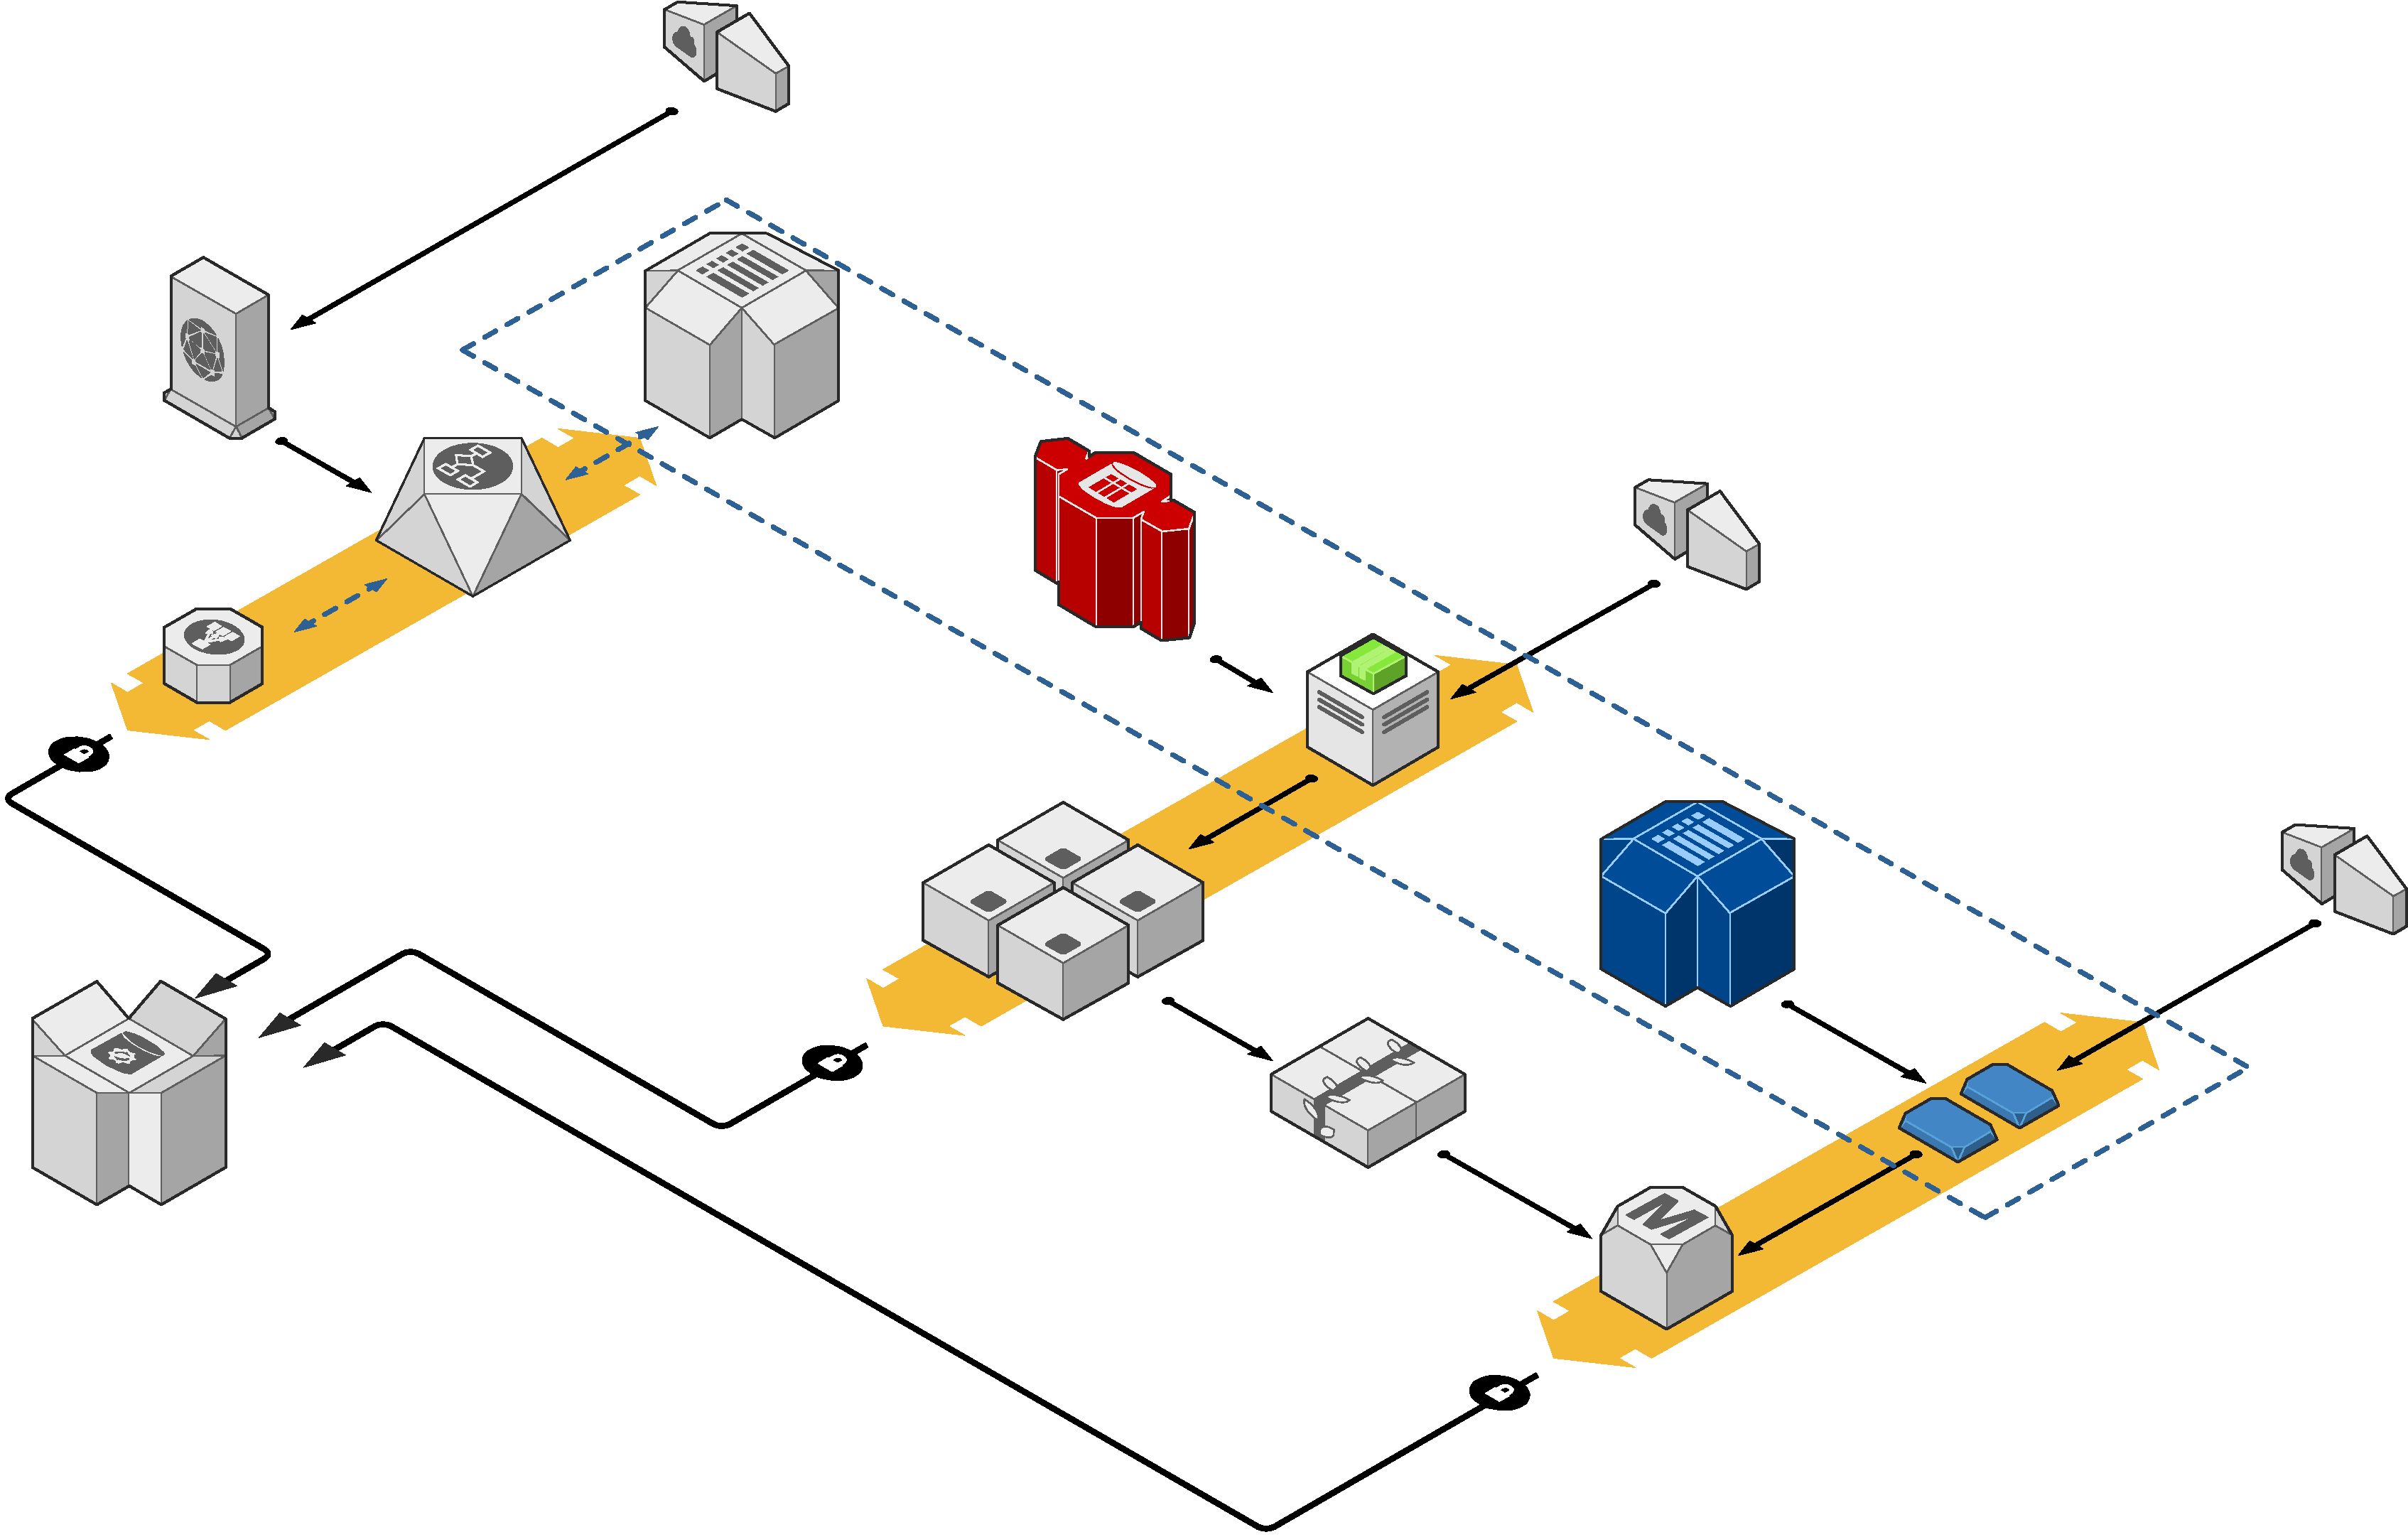
\includegraphics[width=0.4\linewidth, bb=0 0 1626 1038]{example.pdf}
\end{tabular}
\caption{Deja vu? It seems, like I've already seen this diagram.}\label{fig:example-multiple}
\end{figure}

\section{Code, Tables and Quotation}

What about some nice XML? Btw, always \enquote{quote} with the according tag.

\begin{lstlisting}[language=XML]
<note>
  <from>Philipp</from>
  <to>Reader</to>
  <heading>Contact me</heading>
  <email>mail@philippmatth.es</email>
</note>
\end{lstlisting}

\noindent Check out this table! Btw, this may seem a bit confusing, but there is \texttt{tabular}, \texttt{tabularx} or for example also \texttt{longtable}, which is for tables across multiple pages.

\begin{table}[H]
\caption{The caption of your table.}\label{tab:example}
\begin{tabularx}{\textwidth}{{
  >{\hsize=.5\hsize\linewidth=\hsize}X
  >{\hsize=1.5\hsize\linewidth=\hsize}X
}}
\hline
Column 1 & Wider Column 2 \\ \hline \hline
Entry 1.1 & Entry 1.2 \\ \hline
\end{tabularx}
\end{table}

\noindent This was nice. Is there anything missing? File a pull request!


  \newpage

  % use lowercased roman page numbers for the appendix and the bibliography
  \pagenumbering{roman}

  \printbibliography[heading=bibintoc]\label{sec:bibliography}%

  \begin{appendices}
    \tocless\chapter{Appendix A}\label{appendix:a}

  \end{appendices}

\end{document}
